% !TEX root = ../00_thesis.tex

\section{Changing Mode at Runtime}
\label{sec:modeChanges}

\TTW's \feature{Adaptability} relies on switching between different operation modes at runtime. The multi-mode schedule synthesis procedure described in the previous section guarantees that the computed schedules are compatible; that is, persistent applications have the same schedule in different modes~(\cref{sec:multi_mode}).
In this section, we describe the procedure implemented in \TTW to perform the mode changes at runtime.

\TTW controls mode changes using the beacons, sent by the host at the beginning of each round. A beacon contains three elements: the current round $id$, a mode $id$, and a trigger bit $\TB$.
Modes and rounds have unique $id$s with a known mapping of the rounds to the modes. By default, a beacon includes the current mode $id$ and the trigger bit is $0$.
%
A mode change happens in two phases:
First, the change is announced by a beacon including the new mode $id$ (instead of the current one).
In a later round, the \TB is set to $1$, which triggers the mode change; the new mode starts at the end of the round where the \TB is set.
This two step procedure (illustrated in \cref{fig:mode_change}) lets the nodes prepare for an upcoming mode change.%
%
\footnote{\Eg stopping the execution of applications that will be discontinued in the new mode.}
%
Let us denote a beacon by~\beacon and assume $\beacon = \{j, i, 0\}$.
If round $r_j$ (the round with $\id=j$) is mapped to mode \modei, no mode change is announced:
the next round is round $r_{j+1}$ (in the cyclic sequence of rounds associated to mode \mode{i}).
When $\beacon = \{j, k, 0\}$ is sent, the mode change from mode \modei to \mode{k} is announced, but the next round remains based on mode \modei schedule.
Finally, $\beacon = \{j, k, 1\}$ is sent, which triggers the mode change: the next round is the first round of mode \mode{k}.


% The mode change protocol is not specified by \TTW.
Many mode change protocols have been proposed in the literature~(see~\cite{chen2018SafeMC} for an overview). These protocols define the expected behavior of applications in the old and new modes; for example, they specify whether the running applications should be left enough time to complete, or be interrupted by the mode change.
\TTW does not define a specific mode change protocol. Instead, it provides a general strategy to execute mode changes and lets the user define the desired mode change protocol and implement it at the application level.

\begin{figure}
	\centering
	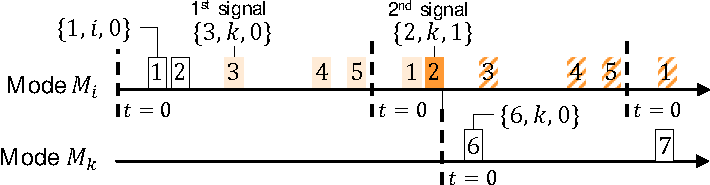
\includegraphics[scale=1]{mode_change}%
	\caption{%
	Example of mode change from mode \mode{i} to \mode{k}.
	\capt{%
	The dashed lines show the start of the mode hyperperiods.
	Each numbered box represents a communication round with its \id.
	The content of some of the host beacons is shown next to the corresponding rounds.
	In $r_3$, the host sends the first signal to change to mode \mode{k}. During this transition phase, the rounds are lightly colored.
	In the dark colored round, the host sets $\TB = 1$. This is the second signal -- directly after this round, mode \mode{k} starts executing.
	Dashed rounds are not executed.
	}
}
\label{fig:mode_change}
\end{figure}

\begin{example}
	Let us consider again the feedback control application from~\cite{mager2019Demo}.
	In this system, we implement a simple mode change protocol: all applications keep running until they are interrupted by a mode change.
%
	When a mode change is announced, a counter (initialized to 10) is appended to the beacon, and decremented with every round.
	The mode change is triggered (\ie \TB is set to~$1$) when the countdown reaches zero.
%
	With this approach, it is sufficient for any node to receive only one out of ten beacons to change mode at the correct time.
	Since the probability of reception of a packet is expected to be above 99\%~\cite{ferrari2011Glossy},
	receiving at least one out of ten beacons will happen with very high probability .
	Thus, this mode change protocol guarantees with very high probability that all the nodes in the system are always executing in the same mode, even in the occurrence of sporadic packet losses; this guarantees conflict-free communication across mode changes.
\end{example}
